%Davide Berardi 2013
%Virtual system development project
%umdevaudio, virtual audio device for the umview virtual machine

\documentclass[a4paper,12pt]{article}

\usepackage{listings}
\usepackage{color}
\usepackage{graphicx}

\definecolor{lcyan}{gray}{0.9}%{rgb}{0.90,0.90,0.80}
\definecolor{purple}{rgb}{0.70,0.0,0.70}

\title{UmDevAudio, Tutorial and examples}
\author{Davide Berardi}
\date{14 settembre 2013}

\begin{document}
	\lstset{
		backgroundcolor=\color{lcyan},
		xleftmargin=.25in,
		linewidth=6.5in,
		showtabs=false,
		showspaces=false,
		%basicstyle=\footnotesize
		%keywordstyle=\color{purple}
		basicstyle=\ttfamily
	}
	\maketitle
	\section{Introduction}
	UmDevAudio is a UmView\footnote{http://wiki.virtualsquare.org/wiki/index.php/UMview} module compatible with tinyalsa\footnote{ALSA and OSS support is still experimental}\footnote{http://github.com/tinyalsa/tinyalsa}.\\
	it can be used for "extending" the actual audio processor like pulseaudio and jack do, but with more control over the real sound card.\\
	for example we can use it to record the stream of data directed to the soundcard;
	so we can record an audio stream which is playing inside a browser.\\
	\section{UmDevAudio modules}
	UmDevAudio is made of two modules, the control module (umdevaudioCtl) and the pcm module (umdevaudioPcm);\\
	the first module is used to control the mixer and the various card-relative options.\\
	the second one is used to control the real data streams and the playing/recording relative options.\\
	\section{Preparing the environment}
	first of all you'll need UmDevAudio.\\
	%qui ci andra' il comando da eseguire, probabilmente git clone ecc
	\begin{lstlisting}[frame=double, language=Bash]
you@pc:~$ git clone umdevaudio
	\end{lstlisting}
	then you must cd inside the new directory (for example UMDEVAUDIO)
	\begin{lstlisting}[frame=double, language=Bash]
you@pc:~$ cd ~/UMDEVAUDIO
	\end{lstlisting}
	then you must place the umview source code inside a directory called "umview" inside the root of the program.\\
	a simple entry in the Makefile is thinked to get the last experimental branch
	\begin{lstlisting}[frame=double, language=Bash]
you@pc:~/UMDEVAUDIO$ make getumview
	\end{lstlisting}
	(or you can just modify the variable UMVIEW in the Makefile)
	then you can continue with a simple make all (the makefile is a wrapper that will do the autoreconf -i; ./configure; make all cycle)
	\begin{lstlisting}[frame=double, language=Bash]
you@pc:~/UMDEVAUDIO$ make all
	\end{lstlisting}
	the next step is installing umview in the system, that is simply accomplished by using again the wrapper Makefile
	\begin{lstlisting}[frame=double, language=Bash]
you@pc:~/UMDEVAUDIO$ sudo make install
	\end{lstlisting}

	\section{Mounting and executing}
	in order to mount and using our virtual sound card we first need to spawn a virtual environment using
	\begin{lstlisting}[frame=double, language=Bash]
you@pc:~$ umview bash
	\end{lstlisting}
	and to add the umdev service
	\begin{lstlisting}[frame=double, language=Bash]
you@pc:~$ um_add_service umdev
	\end{lstlisting}
	now we can mount our modules on the designated card with
	\begin{lstlisting}[frame=double, language=Bash]
you@pc:~$ mount -t umdevaudioCtl [-o card:<cardNo>] none\
	/dev/snd/controlC<cardNo>
you@pc:~$ mount -t umdevaudioCtl [-o card:<cardNo>] none\
	/dev/snd/pcmC<cardNo>D<deviceNo><'p'or'c'>
	\end{lstlisting}
	for example we can mount on card 2 with the command
	\begin{lstlisting}[frame=double, language=Bash]
you@pc:~$ mount -t umdevaudioCtl -o card:2 none\
	/dev/snd/controlC2
you@pc:~$ mount -t umdevaudioCtl -o card:2 none\
	/dev/snd/pcmC2D0p
	\end{lstlisting}

	umdevaudio have some options to configure the virtual soundcard like:
	\begin{itemize}
	\item card:cardNo										(like card:2)
	\item version:soundProtocolVersion	(like version:2.0.10, for alpha test for soundcards)
	\item controls:number								(like controls:4 for 4 mixers)
	\item playcap:'p'or'c'							(like playcap:p for playback devices)
	\item configrc:path									(like config:~/.umaudiorc for configure the min/max framerate etc)
	\item file:path											(like file:~/test.raw to set the input/output file)
	\end{itemize}

	\section{VirtualSuite}
	Virtual Suite is a simple script to simplifying the mount process of all required modules of umdevaudio.\\
	to use it simply use
	\begin{lstlisting}[frame=double, language=Bash]
you@pc:~/UMDEVAUDIO$ ./VirtualSuite [cardno][options]
	\end{lstlisting}
	where options can be one or more of the followings
	\begin{itemize}
	\item -v / --protocol			sound protocol p.e. 2.0.2
	\item -m / --mixer-size 	number of control's mixer
	\item -c / --control			control module mount path
	\item -p / --pcm-path			pcm module mount path
	\item --virtual-conf			virtual configuration file (contains options like min/max framerate etc)
	\item -P / --playcap			pcm is mounted as playback or capture
	\item -o / --outfile			path to the file on which the stream is recorded
	\end{itemize}


	\section{Examples}
	\subsection{record the audio stream in a raw file}
 you'll start with initializing the environment with mounting our virtual card as the card 2 (for example)
	\begin{lstlisting}[frame=double, language=Bash]
you@pc:~/UMDEVAUDIO$ ./VirtualSuite 2 -P p
you@umview ~/UMDEVAUDIO => 
	\end{lstlisting}
	next you can play the stream using tinyplay

	\begin{lstlisting}[frame=double, language=Bash]
you@umview ~/UMDEVAUDIO => tinyplay <wavfile> -D 2 0
	\end{lstlisting}

	now you'll have your recorded file on /tmp/outBuffer\\
	%screen con hex
	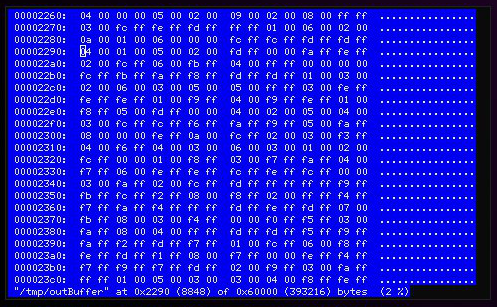
\includegraphics[scale=0.90]{hexer_done.png}
	so you can just use aplay (outside the virtual machine, or on your real card!) to play it

	\begin{lstlisting}[frame=double, language=Bash]
you@pc:~$ aplay -M -t raw -f cd -r 44100 /tmp/outBuffer
	\end{lstlisting}

	\subsection{put a file as the sound recorded from the mic}
	you'll start with initializing the environment with mounting our virtual card as the card 2 (for example)
	\begin{lstlisting}[frame=double, language=Bash]
you@pc:~/UMDEVAUDIO$ ./VirtualSuite 2 -P c
you@umview ~/UMDEVAUDIO => 
	\end{lstlisting}
	next you can "record" the input raw file (by default /tmp/outBuffer) with tinycap

	\begin{lstlisting}[frame=double, language=Bash]
you@umview ~/UMDEVAUDIO => tinycap <out wav file> -D 2 -d 0
	\end{lstlisting}

	so now you'll have your output file recorded.\\
	you can test it with aplay (on your real card!)\\

	\begin{lstlisting}[frame=double, language=Bash]
you@pc:~$ aplay <out wav file>
	\end{lstlisting}

\end{document}
